\documentclass[english,,man]{apa6}
\usepackage{lmodern}
\usepackage{amssymb,amsmath}
\usepackage{ifxetex,ifluatex}
\usepackage{fixltx2e} % provides \textsubscript
\ifnum 0\ifxetex 1\fi\ifluatex 1\fi=0 % if pdftex
  \usepackage[T1]{fontenc}
  \usepackage[utf8]{inputenc}
\else % if luatex or xelatex
  \ifxetex
    \usepackage{mathspec}
  \else
    \usepackage{fontspec}
  \fi
  \defaultfontfeatures{Ligatures=TeX,Scale=MatchLowercase}
\fi
% use upquote if available, for straight quotes in verbatim environments
\IfFileExists{upquote.sty}{\usepackage{upquote}}{}
% use microtype if available
\IfFileExists{microtype.sty}{%
\usepackage{microtype}
\UseMicrotypeSet[protrusion]{basicmath} % disable protrusion for tt fonts
}{}
\usepackage{hyperref}
\hypersetup{unicode=true,
            pdftitle={LAB: Linguistic Annotated Bibliography -- A searchable portal for normed database information},
            pdfauthor={Erin M. Buchanan, K. D. Valentine, \& Nicholas P. Maxwell},
            pdfkeywords={database, stimuli, online portal, megastudy, trends},
            pdfborder={0 0 0},
            breaklinks=true}
\urlstyle{same}  % don't use monospace font for urls
\ifnum 0\ifxetex 1\fi\ifluatex 1\fi=0 % if pdftex
  \usepackage[shorthands=off,main=english]{babel}
\else
  \usepackage{polyglossia}
  \setmainlanguage[]{english}
\fi
\usepackage{graphicx,grffile}
\makeatletter
\def\maxwidth{\ifdim\Gin@nat@width>\linewidth\linewidth\else\Gin@nat@width\fi}
\def\maxheight{\ifdim\Gin@nat@height>\textheight\textheight\else\Gin@nat@height\fi}
\makeatother
% Scale images if necessary, so that they will not overflow the page
% margins by default, and it is still possible to overwrite the defaults
% using explicit options in \includegraphics[width, height, ...]{}
\setkeys{Gin}{width=\maxwidth,height=\maxheight,keepaspectratio}
\IfFileExists{parskip.sty}{%
\usepackage{parskip}
}{% else
\setlength{\parindent}{0pt}
\setlength{\parskip}{6pt plus 2pt minus 1pt}
}
\setlength{\emergencystretch}{3em}  % prevent overfull lines
\providecommand{\tightlist}{%
  \setlength{\itemsep}{0pt}\setlength{\parskip}{0pt}}
\setcounter{secnumdepth}{0}
% Redefines (sub)paragraphs to behave more like sections
\ifx\paragraph\undefined\else
\let\oldparagraph\paragraph
\renewcommand{\paragraph}[1]{\oldparagraph{#1}\mbox{}}
\fi
\ifx\subparagraph\undefined\else
\let\oldsubparagraph\subparagraph
\renewcommand{\subparagraph}[1]{\oldsubparagraph{#1}\mbox{}}
\fi

%%% Use protect on footnotes to avoid problems with footnotes in titles
\let\rmarkdownfootnote\footnote%
\def\footnote{\protect\rmarkdownfootnote}


  \title{LAB: Linguistic Annotated Bibliography -- A searchable portal for normed
database information}
    \author{Erin M. Buchanan\textsuperscript{1}, K. D. Valentine\textsuperscript{2},
\& Nicholas P. Maxwell\textsuperscript{1}}
    \date{}
  
\shorttitle{Linguistic Bibliography}
\affiliation{
\vspace{0.5cm}
\textsuperscript{1} Missouri State University\\\textsuperscript{2} University of Missouri}
\keywords{database, stimuli, online portal, megastudy, trends}
\usepackage{csquotes}
\usepackage{upgreek}
\captionsetup{font=singlespacing,justification=justified}

\usepackage{longtable}
\usepackage{lscape}
\usepackage{multirow}
\usepackage{tabularx}
\usepackage[flushleft]{threeparttable}
\usepackage{threeparttablex}

\newenvironment{lltable}{\begin{landscape}\begin{center}\begin{ThreePartTable}}{\end{ThreePartTable}\end{center}\end{landscape}}

\makeatletter
\newcommand\LastLTentrywidth{1em}
\newlength\longtablewidth
\setlength{\longtablewidth}{1in}
\newcommand{\getlongtablewidth}{\begingroup \ifcsname LT@\roman{LT@tables}\endcsname \global\longtablewidth=0pt \renewcommand{\LT@entry}[2]{\global\advance\longtablewidth by ##2\relax\gdef\LastLTentrywidth{##2}}\@nameuse{LT@\roman{LT@tables}} \fi \endgroup}


\DeclareDelayedFloatFlavor{ThreePartTable}{table}
\DeclareDelayedFloatFlavor{lltable}{table}
\DeclareDelayedFloatFlavor*{longtable}{table}
\makeatletter
\renewcommand{\efloat@iwrite}[1]{\immediate\expandafter\protected@write\csname efloat@post#1\endcsname{}}
\makeatother
\usepackage{lineno}

\linenumbers

\authornote{Erin M. Buchanan is an Associate Professor of
Quantitative Psychology at Missouri State University. K. D. Valentine is
a Ph.D.~candidate at the University of Missouri. Nicholas P. Maxwell
received his master's degree from Missouri State University and is now a
Ph.D.~candidate at the University of Southern Mississippi. We thank
Michael T. Carr, Farren E. Bankovich, Samantha D. Saxton, and Emmanuel
Segui for their help with the original data processing, and William
Padfield, Abigial Van Nuland, and Addie Wikowsky for their help with the
application development for the website.

Correspondence concerning this article should be addressed to Erin M.
Buchanan, 901 S. National Ave, Springfield, MO 65897. E-mail:
\href{mailto:erinbuchanan@missouristate.edu}{\nolinkurl{erinbuchanan@missouristate.edu}}}

\abstract{
This article presents the Linguistic Annotated Bibliography (LAB) as a
searchable web portal to quickly and easily access reliable database
norms, related programs, and variable calculations. These publications
were coded by language, number of stimuli, stimuli type (i.e., words,
pictures, symbols), keywords (i.e., frequency, semantics, valence), and
other useful information. This tool not only allows researchers to
search for the specific type of stimuli needed for experiments, but also
permits the exploration of publication trends across 100 years of
research. Details about the portal creation and use are outlined, as
well as various analyses of change in publication rates and keywords. In
general, advances in computational power have allowed for the increase
in dataset size in the recent decades, in addition to an increase in the
number of linguistic variables provided in each publication.


}

\usepackage{amsthm}
\newtheorem{theorem}{Theorem}[section]
\newtheorem{lemma}{Lemma}[section]
\theoremstyle{definition}
\newtheorem{definition}{Definition}[section]
\newtheorem{corollary}{Corollary}[section]
\newtheorem{proposition}{Proposition}[section]
\theoremstyle{definition}
\newtheorem{example}{Example}[section]
\theoremstyle{definition}
\newtheorem{exercise}{Exercise}[section]
\theoremstyle{remark}
\newtheorem*{remark}{Remark}
\newtheorem*{solution}{Solution}
\begin{document}
\maketitle

The advance of computational ability and the Internet have propelled
research into an era of \enquote{big data} that has interesting
implications for the field of psycholinguistics, as well as other
experimental areas that use normed stimuli for their research.
Traditionally, stimuli used for experimental psycholinguistics research
were first normed through small in-house pilot studies, which were then
used in many subsequent projects. While economic, the results from these
studies could be potentially misleading, as the results may be due to
the stimuli, rather than experimental manipulation. Small individual lab
norming projects may be tied to a lack of funding, time, computational
power, or even interest in studying phenomena at the stimuli level. Now,
we have the capability to collect, analyze, and publish large datasets
for research into memory models (Cree, McRae, \& McNorgan, 1999; Moss,
Tyler, \& Devlin, 2002; Rogers \& McClelland, 2004; Vigliocco, Vinson,
Lewis, \& Garrett, 2004), aphasias (Vinson, Vigliocco, Cappa, \& Siri,
2003), featural probability (Cree \& McRae, 2003; McRae, Sa, \&
Seidenberg, 1997; Pexman, Holyk, \& Monfils, 2003), valence (Dodds,
Harris, Kloumann, Bliss, \& Danforth, 2011; Vo et al., 2009; Warriner,
Kuperman, \& Brysbaert, 2013), and reading speeds and priming (Balota et
al., 2007; Cohen-Shikora, Balota, Kapuria, \& Yap, 2013; Hutchison et
al., 2013; Keuleers, Lacey, Rastle, \& Brysbaert, 2012) to name a small
subset of research avenues.

Big data has manifested in psycholinguistics over the last decade in the
form of grant funded megastudies to collect and analyze large text
corpora (i.e., the SUBTLEX projects) or to examine numerous word
properties (i.e., the Lexicon projects). The SUBTLEX projects were
designed to analyze frequency counts for concepts across large corpora
sizes using subtitles as a substitute for natural speech. The
investigation of these measures was first spurred by the realization
that word frequency is an important predictor of naming and lexical
decision times (Balota, Cortese, Sergent-Marshall, Spieler, \& Yap,
2004; Rayner \& Duffy, 1986). While previous measures of frequency
(i.e., Baayen, Piepenbrock, Gulikers, \& Linguistic Data Consortium,
1995; Burgess \& Livesay, 1998; Kučera \& Francis, 1967) were based on
large one million+ word corpora, they were poor predictors of response
latencies (Balota et al., 2004; Brysbaert \& New, 2009; Zevin \&
Seidenberg, 2002). Further, Brysbaert and New (2009) indicate the
importance of corpus' characteristics for psycholinguistic studies, as
the underlying source of the text data matters (Internet versus
subtitles), as well as the contextual diversity of the data (i.e.,
number of occurrences across sources; Adelman, Brown, \& Quesada, 2006).
Not only has Brysbaert and New (2009)'s work been included in newer
lexical studies (Hutchison et al., 2013; Yap, Tan, Pexman, \&
Hargreaves, 2011), but SUBTLEX projects have been published in Dutch
(Keuleers, Brysbaert, \& New, 2010), Greek (Dimitropoulou, Duñabeitia,
Avilés, Corral, \& Carreiras, 2010), Spanish (Cuetos, Glez-Nosti,
Barbon, \& Brysbaert, 2011), Chinese (Cai \& Brysbaert, 2010), French
(New, Brysbaert, Veronis, \& Pallier, 2007), British English (Heuven,
Mandera, Keuleers, \& Brysbaert, 2014), Polish (Mandera, Keuleers,
Wodniecka, \& Brysbaert, 2015), and German (Brysbaert et al., 2011).

The Lexicon projects involved creating large databases of mono- and
multisyllabic words to assist in the creation of controlled experimental
stimuli sets for future experiments. These databases contain lexical
decision and naming response latencies, as well as typical word confound
variables such as orthographic neighborhood, phonological, and
morphological characteristics. While the English Lexicon Project (Balota
et al., 2007) is the most cited of the lexicons, other languages include
Chinese (Sze, Rickard Liow, \& Yap, 2014; Tse et al., 2017), Malay (Yap,
Rickard Liow, Jalil, \& Faizal, 2010), Dutch (Keuleers et al., 2010),
and British English (Keuleers et al., 2012). Similar lexical database
publications can be found in the literature covering French (Lété,
Sprenger-Charolles, \& Colé, 2004), Italian (Barca, Burani, \& Arduino,
2002), Arabic (Boudelaa \& Marslen-Wilson, 2010), and Portuguese (Soares
et al., 2014).

The availability of big data has augmented the psycholinguistic
literature, but these projects are certainly time consuming due to the
amount of participant data required to achieve reliable and stable
norms. A solution to large data collection lies in several avenues of
easily obtainable data. First, Amazon's Mechanical Turk, an online crowd
sourcing avenue that allows researchers to pay users to complete
questionnaires, can be a reliable, diverse participant pool made
available at very low cost (Buhrmester, Kwang, \& Gosling, 2011; Mason
\& Suri, 2012). Researchers can pre-screen for specific populations, as
well as post-screen surveys for incomplete or inappropriate responses
(Buchanan \& Scofield, 2018), thus saving time and money with the
elimination of poor data. Because of the popularity of Mechanical Turk,
large amounts of data can be collected in shorter time periods than
traditional experiments. Mechanical Turk has been used to collect data
for semantic word pair norms (Buchanan, Holmes, Teasley, \& Hutchison,
2013), age of acquisition ratings (Kuperman, Stadthagen-Gonzalez, \&
Brysbaert, 2012), concreteness ratings (Brysbaert, Warriner, \&
Kuperman, 2014), past tense information (Cohen-Shikora et al., 2013),
and valence and arousal ratings (Dodds et al., 2011; Warriner et al.,
2013). Additionally, in a similar vein to the SUBTLEX projects,
linguistic data has been mined from open source data, such as the New
York Times, music lyrics, and Twitter (Dodds et al., 2011; Kloumann,
Danforth, Harris, Bliss, \& Dodds, 2012). Finally, De Deyne, Navarro,
and Storms (2013) have seen success in setting up a special website
(www.smallworldofwords.com) to gamify the collection of word pair
association norms.

The evolution of big data provides exciting opportunities for
exploration into psycholinguistics, and this article features the trends
in publications of normed datasets across the literature, allowing for a
large-scale picture of the developments of trends in psychological
stimuli. Historically, these norms have been published in journals
connected to the Psychonomic Society, such as Behavior Research Methods,
Psychonomic Monograph Supplements, and Perception and Psychophysics. The
Psychonomic Society once hosted an electronic database that contained
the links to these norms, as well as a search tool to find information
about previously published works (Vaughan, 2004). The sale of the
society journals to Springer publications has improved journal
visibility and user-friendly access, but also has left a need for an
indexed list of database publications that span multiple keywords and
journal websites. Other researchers have started a similar task,
publishing the Language Goldmine, an online searchable database of
linguistic resources (List, Winter, \& Wedel, n.d.). Within the Language
Goldmine, users can find over two-hundred citations for linguistic
resources, which are mostly corpora. This article extends that resource
by: 1) presenting a searchable, cataloged database of normed stimuli and
related materials for a wide range of experimental research, and 2) to
examine trends in the publications of these articles to assess the big
data movement within cognitive psychology.

\hypertarget{website}{%
\section{Website}\label{website}}

This manuscript was written with \emph{R} markdown and \emph{papaja}
(Aust \& Barth, 2017) and can be found at \url{https://osf.io/9bcws/}.
Readers can find the LAB's website by going to
\url{http://www.wordnorms.com}, and the source files for the website can
be found at \url{https://github.com/doomlab/wordnorms}. From the
webpage, the top navigation bar includes a link to direct the reader to
the LAB page. On the LAB page, we have included a purpose statement and
several summary options. First, the two variable tables include summary
descriptions about the stimuli and keyword (tag) variables in this study
using an embedded Shiny application. Shiny is an open source graphical
user interface \emph{R} package that allows researchers to build
interactive web applications (Chang, Cheng, Allaire, Xie, \& McPherson,
2017). These apps connect to the LAB database and display the current
sample size \emph{N}, minimum, maximum, mean standard deviation, and
correlation across years for each variable, when appropriate. The
advantage to using Shiny apps is dynamic updating of the database, so as
new information is added, the app will display the most current
statistics, while this paper represents a static point in the database
development. The entire dataset can be viewed and filtered based on
keyword, language, and stimuli type. This search app allows for multiple
filter options, so a person may drill down into very specific search
criteria. Underneath the search functions, yearly trend visualization
and descriptive statistics may be found including frequency tables of
stimuli and keywords. Finally, the complete database in .csv format can
be downloaded. Specific features will be outlined below in relation to
the database creation.

The website includes more information on versioning of the dataset for
users to reference, along with instructions on how and what others can
contribute to the LAB. Viewers can suggest articles that should be
included in the dataset by using the online Mendeley group (requires
login and account) at
\url{https://www.mendeley.com/community/the-lab-linguistic-annotated-bibliography/}
or using the email link included in the top right corner of the website.
Mendeley is free reference software that allows for open source groups
to collaborate on curating reference lists. Additionally, we have
provided a BibTex reference file linked on the website that can be
imported into most reference software programs.

\hypertarget{database-methods}{%
\section{Database Methods}\label{database-methods}}

\hypertarget{materials}{%
\subsection{Materials}\label{materials}}

Bradshaw (1984) and Proctor and Vu (1999)'s lists of database
information were used as starting points for collection of research
articles. We searched \emph{Academic Search Premier}, \emph{PsycInfo},
and \emph{ERIC} through the EBSCO host system, as well as \emph{Google
Scholar} and \emph{PLoS One} to find other relevant articles using the
following keywords: \emph{corpus, linguistic database, linguistic norms,
norms}, and \emph{database}. Additionally, since a large number of the
original articles were hosted by the Psychonomic Society, the Springer
website was searched with these terms that covered the newer editions of
\emph{Behavior Research Methods} and \emph{Memory \& Cognition}. We then
filtered for articles that met the following criteria: 1) contained
database information as supplemental material, 2) demonstrated programs
related to building research stimuli using normed databases, or 3)
generated new calculations of lexical variables. Research articles that
used normed databases in experimental design or tested those variables
validity/reliability were excluded if they did not include new database
information. Additional articles were found while coding initial
publications by searching citations for stimuli selection. For example,
the Snodgrass and Vanderwart (1980) norms were cited in multiple newer
articles on line drawings, and therefore this article was subsequently
entered into the database. Last, we consulted the Language Goldmine and
included all citations from this resource that could still be accessed
(List et al., n.d.). At the time of writing, 884 articles, books,
websites, and technical reports were included in the following analyses.

\hypertarget{coding-procedure}{%
\subsection{Coding Procedure}\label{coding-procedure}}

The tables with summaries from Bradshaw (1984) and Proctor and Vu (1999)
were consulted for a starting point for data coding. Next, the first
round of articles found (approximately 100) were analyzed to determine
information that would be pertinent to a user who wished to search for
normed stimuli. Based on these reviews and lab discussions, we coded the
following information from each article: 1) journal information, 2)
stimuli types, 3) stimuli language, 4) program or corpus name, 5)
keywords, which we refer to as tags, 6) special populations, and 7)
other notes that did not fit into those categories. Each piece of
information is detailed below. In some instances, codes were not used as
frequently as expected based on these initial discussions, but were
included to allow more specificity in searching, as well as the
flexibility to include those options for articles subsequently added to
the database.

\hypertarget{journal-information}{%
\subsubsection{Journal Information}\label{journal-information}}

Each article was coded with the citation information, and a complete
list of citations can be found on the website portal by going to the
search data section. All author last names are listed, along with
publication year, article title, journal title, volume, page numbers,
and digital object identifier (DOI) when available. This information is
listed in citation format in the Shiny app and separated into columns in
the downloadable data for easier sorting and searching. A complete list
of publication sources and percentages can be found online by using the
frequency statistics link.

\hypertarget{stimuli-types}{%
\subsubsection{Stimuli Types}\label{stimuli-types}}

While this publication was originally intended for traditional
linguistic database norms, other types of experimental stimuli used in
concept studies were apparent after background review. Therefore,
stimuli were coded based on the dominant description from the article
(i.e., although heteronyms are words and word pairs, they were coded
specifically as heteronyms). The number of stimuli presented in the
appendix or database was coded with the stimuli if it was available.
Generally, programs, corpora, and experimental creation tools did not
include this information, which are the majority of the \enquote{other}
stimuli category. Because many articles included two types of stimuli,
or references to different articles where stimuli were selected from,
two options for stimuli were included.

Therefore, the total values for number of stimuli do not add up to the
number of articles in the database because of multiple instances in
articles or no stimuli for program descriptions. Table
\ref{tab:stim-table} includes a stimuli list, the number of times that
each stimuli was used, percentage of the total stimuli codes, minimum,
maximum, the mean and standard deviation of the number of those stimuli.
Brief variable descriptions are provided online under variable tables.
Researchers often cited specific previous works where stimuli were
selected from, and these references were included, which can be found in
the downloaded data. Table \ref{tab:stim-table} is included dynamically
online under \enquote{view the variable table}" and \enquote{view the
frequency table}.

\begin{table}[tbp]
\begin{center}
\begin{threeparttable}
\caption{\label{tab:stim-table}Stimuli Descriptive Statistics}
\small{
\begin{tabular}{lcccccc}
\toprule
Stimuli & $N$ & Percent & Min & Max & $M$ & $SD$\\
\midrule
Anagrams & \ \ 6 & 0.6 & \ \  80 & \ \ \ \ \ \ 378 & \ \ \ \  229.00 & \ \ \ \ \ \ 210.72\\
Categories & 33 & 3.4 & \ \ \ \ 4 & \ \ \ \ \ \ 240 & \ \ \ \ \ \ 46.32 & \ \ \ \ \ \  51.61\\
Characters & 21 & 2.1 & \ \  48 & \ \ \ \ 80651 & \ \ \ \ 8458.37 & \ \ \ \ 19210.92\\
Cloze/Sentences & 35 & 3.6 & \ \ \ \ 5 & \ \ \ \  1998 & \ \ \ \  353.66 & \ \ \ \ \ \ 376.01\\
Color drawings & 11 & 1.1 & \ \ 200 & \ \ \ \ \ \ 750 & \ \ \ \  406.00 & \ \ \ \ \ \ 225.00\\
Corpus & 116 & 11.9 & 40000 & 700000000 & 72787972.48 & 155024616.77\\
Homo/Heterographs & 11 & 1.1 & \ \  20 & \ \ \ \ \ \ 566 & \ \ \ \  165.00 & \ \ \ \ \ \ 165.38\\
Homo/Heteronyms & \ \ 5 & 0.5 & \ \ 114 & \ \ \ \ \ \ 578 & \ \ \ \  343.75 & \ \ \ \ \ \ 251.45\\
Homo/Heterophones & \ \ 4 & 0.4 & \ \  40 & \ \ \ \ \ \ 207 & \ \ \ \  148.00 & \ \ \ \ \ \  93.66\\
Letters & 57 & 5.8 & \ \ \ \ 9 & \ \ \ \  8836 & \ \ \ \  669.88 & \ \ \ \  1564.37\\
Line drawings & 44 & 4.5 & \ \  22 & \ \ \ \ \ \ 520 & \ \ \ \  253.93 & \ \ \ \ \ \ 130.51\\
Names & \ \ 8 & 0.8 & \ \ 126 & \ \ \ \ 10000 & \ \ \ \ 2644.17 & \ \ \ \  4080.78\\
Other & 85 & 8.7 & \ \ \ \ 1 & \ \ \ \  3061 & \ \ \ \  666.13 & \ \ \ \ \ \ 876.87\\
Phonemes & \ \ 9 & 0.9 & 10000 & \ \ \ \ 10000 & \ \  10000.00 & \ \ \ \ \ \ \ \ \ \ NA\\
Pictures & 74 & 7.6 & \ \ \ \ 2 & \ \ \ \  2941 & \ \ \ \  431.26 & \ \ \ \ \ \ 480.61\\
Pseudowords & 15 & 1.5 & \ \  30 & \ \ \ \ 40481 & \ \  14004.36 & \ \ \ \ 15223.04\\
Sentences & \ \ 7 & 0.7 & \ \ \ \ 9 & \ \ \ \ \ \ 240 & \ \ \ \  101.29 & \ \ \ \ \ \  90.46\\
Sounds & 15 & 1.5 & \ \  22 & \ \ \ \  2159 & \ \ \ \  462.58 & \ \ \ \ \ \ 672.79\\
Syllables & 11 & 1.1 & \ \  20 & \ \  303636 & \ \  44868.80 & \ \  100922.91\\
Symbols/Icons & \ \ 9 & 0.9 & \ \  68 & \ \ \ \ \ \ 600 & \ \ \ \  294.60 & \ \ \ \ \ \ 195.07\\
Word Pairs & 28 & 2.9 & \ \  40 & \ \ \ \ 72186 & \ \ \ \ 8076.83 & \ \ \ \ 20871.25\\
Words & 374 & 38.2 & \ \  10 & 33500000 & \ \ 115731.45 & \ \ 1843018.04\\
\bottomrule
\end{tabular}
}
\end{threeparttable}
\end{center}
\end{table}

\hypertarget{stimuli-language}{%
\subsubsection{Stimuli Language}\label{stimuli-language}}

The language of the stimuli set was coded by starting with the most
common languages from the first articles surveyed, and others were added
as it was apparent that several norms were present for that language
(such as Japanese, Dutch, and Greek). A multiple category was created
for for datasets with more than one set of language norms, with more
information about the languages available provided in the notes column.
If the stimuli were non-linguistic selections, like pictures and line
drawings, the language of the participants used to norm the set was
used, which was commonly English. In order to help distinguish these
norms, a column was added that denoted non-linguistic norms (coded as 0
for linguistic, 1 for non-linguistic). For each language, the Glottolog
codes were added in a separate column to help identify them
(Hammarstrom, Forkel, \& Haspelmath, n.d.). One potential limitation of
the LAB was that English is the first language for the authors; however,
translation tools were used to code sources found in other languages.
Table \ref{tab:lang-table} indicates language frequencies and
percentages, and the online version can be found by clicking the view
frequency statistics link.

\begin{table}[tbp]
\begin{center}
\begin{threeparttable}
\caption{\label{tab:lang-table}Language Descriptive Statistics}
\begin{tabular}{lcc}
\toprule
Language & $N$ & Percent\\
\midrule
Arabic & \ \ 8 & 0.9\\
British English & 25 & 2.8\\
Chinese & 33 & 3.7\\
Dutch & 18 & 2.0\\
English & 470 & 53.2\\
French & 46 & 5.2\\
German & 37 & 4.2\\
Greek & \ \ 6 & 0.7\\
Italian & 20 & 2.3\\
Japanese & 14 & 1.6\\
Multiple & 86 & 9.7\\
Polish & \ \ 6 & 0.7\\
Portuguese & 18 & 2.0\\
Russian & \ \ 6 & 0.7\\
Spanish & 61 & 6.9\\
\bottomrule
\addlinespace
\end{tabular}
\begin{tablenotes}[para]
\normalsize{\textit{Note.} Languages with less than five entries were excluded for publication space purposes.}
\end{tablenotes}
\end{threeparttable}
\end{center}
\end{table}

\hypertarget{programcorpus-name}{%
\subsubsection{Program/corpus name}\label{programcorpus-name}}

In many instances, megastudies are often named, such as the English
Lexicon Project (Balota et al., 2007), for easier reference. This
information was included in the dataset, which will also help
researchers with the stimuli references as described above. For example,
a newer study may reference using the BOSS database (Brodeur,
Dionne-Dostie, Montreuil, \& Lepage, 2010) and having that information
would make searching for the original article easier by using the corpus
name column (especially in instances the dataset name is not listed in
the article title). The names of programs or tools were also entered,
such as NIM (Guasch, Boada, Ferré, \& Sánchez-Casas, 2013), a newer
stimuli selection tool for psycholinguistic studies.

\hypertarget{keyword-tags}{%
\subsubsection{Keyword Tags}\label{keyword-tags}}

Keyword tags are the majority of the database, as they allow for the
best understanding of trends and availability of stimuli. Tables
\ref{tab:tag-table} and \ref{tab:tag-table2} portray a list of tags,
frequencies, percentages, and correlations (described below) for tags
with sample sizes greater than 10. Tag descriptions are provided online
under tag table. Each article was coded with tags based on the
description of the accessible data, and a single article may have
multiple tags. However, due to the cumulative nature of database
research, this tagging system does not mean that each article collected
that particular type of data. The most common example of this
distinction occurs when data was combined across sources, but presented
in a new article. The Maki, McKinley, and Thompson (2004) semantic
distance norms also included values from the South Florida Free
Association norms (Nelson, McEvoy, \& Schreiber, 2004), and Latent
Semantic Analysis (Landauer \& Dumais, 1997). Therefore, this article
was coded with association and semantics, even though the association
norms were not collected in that paper. As described above, some small
frequency tags were used because of the initial pass through newer
articles, but these were left in the database because of their
specificity, and they can be used in future additions.

\begin{table}[tbp]
\begin{center}
\begin{threeparttable}
\caption{\label{tab:tag-table}Tag Descriptive Statistics}
\small{
\begin{tabular}{lccc}
\toprule
Stimuli & $N$ & Percent & $r$\\
\midrule
Age of Acquisition & 107 & 4.9 & .134\\
Ambiguity/Word Meaning & 31 & 1.4 & -.076\\
Arousal & 62 & 2.9 & .173\\
Association & 86 & 4.0 & -.336\\
Category & 48 & 2.2 & -.068\\
Complexity & 22 & 1.0 & NA\\
Concreteness & 73 & 3.4 & .001\\
Confusion Matrices & 18 & 0.8 & NA\\
Context & 14 & 0.6 & NA\\
Dominance & 33 & 1.5 & .045\\
Familiarity & 141 & 6.5 & .116\\
Frequency & 252 & 11.6 & .005\\
Grapheme-Phoneme Correspondence & 18 & 0.8 & NA\\
Identification & 17 & 0.8 & NA\\
Identification - Lexical Decision & 16 & 0.7 & NA\\
Identification - Naming & 50 & 2.3 & .098\\
Image Agreement & 24 & 1.1 & NA\\
Imageability & 95 & 4.4 & .023\\
Letters & 70 & 3.2 & .081\\
\bottomrule
\addlinespace
\end{tabular}
}
\begin{tablenotes}[para]
\normalsize{\textit{Note.} Correlation refers to the correlation between publication year and the frequency of a given tag when sample size is greater than 30.}
\end{tablenotes}
\end{threeparttable}
\end{center}
\end{table}

\begin{table}[tbp]
\begin{center}
\begin{threeparttable}
\caption{\label{tab:tag-table2}Tag Descriptive Statistics Continued}
\small{
\begin{tabular}{lccc}
\toprule
Stimuli & $N$ & Percent & $r$\\
\midrule
Meaningfulness & 48 & 2.2 & -.162\\
Morphology & 24 & 1.1 & NA\\
Name Agreement & 47 & 2.2 & .090\\
Orthographic Neighborhood & 56 & 2.6 & .112\\
Part of Speech & 67 & 3.1 & .095\\
Phonemes & 62 & 2.9 & .126\\
Phonological Neighborhood & 38 & 1.8 & .111\\
Pronunciation & 16 & 0.7 & NA\\
Response Times & 78 & 3.6 & .069\\
Recall & 19 & 0.9 & NA\\
Recognition & 18 & 0.8 & NA\\
Semantics & 109 & 5.0 & .056\\
Sensory/Motor & 39 & 1.8 & .071\\
Similarity & 21 & 1.0 & NA\\
Syllables & 64 & 3.0 & .148\\
Syntax & 23 & 1.1 & NA\\
Typicality & 25 & 1.2 & NA\\
Valence/Emotion & 115 & 5.3 & .156\\
Visual Complexity & 40 & 1.8 & .090\\
\bottomrule
\addlinespace
\end{tabular}
}
\begin{tablenotes}[para]
\normalsize{\textit{Note.} Correlation refers to the correlation between publication year and the frequency of a given tag when sample size is greater than 30.}
\end{tablenotes}
\end{threeparttable}
\end{center}
\end{table}

\hypertarget{special-populations}{%
\subsubsection{Special Populations}\label{special-populations}}

While coding articles, it became apparent that a subset of the normed
data was tested on specific special populations. Consequently,
demographic data such as gender, age, ethnicity, and grade school year
were listed as described in the article (i.e., if ages were used, age
was listed, but if grade year was used, it was listed rather than
translating to specific ages).

\hypertarget{othernotes}{%
\subsubsection{Other/Notes}\label{othernotes}}

Lastly, places for more description were included for tags or variables
not frequently used, which was especially useful for program
descriptions, as well as descriptions of specific types of stimuli
(i.e., CVC trigrams). In several instances, notes that appeared
frequently were moved to tags (such as similarity) after the database
had several hundred articles sampled. All information described above
without a specific table (special populations, other, program/corpus
names, and journal information) can be found by downloading the complete
dataset.

\hypertarget{results-and-discussion}{%
\section{Results and Discussion}\label{results-and-discussion}}

\hypertarget{journals}{%
\subsection{Journals}\label{journals}}

Journal results, unsurprisingly, show that the wealth of data was
published in \emph{Behavior Research Methods} (57.6\% combined across
name changes).The next largest publishers of articles were
\emph{Psychonomic Monograph Supplements} (2.1\%), \emph{Journal of
Verbal Learning and Verbal Behavior} (1.7\%), \emph{Psychonomic Science}
(1.7\%), \emph{Journal of Experimental Psychology} (combined across
subjournals, 2.5\%), \emph{Perception \& Psychophysics} (1.5\%),
\emph{Memory \& Cognition} (1.4\%), \emph{Bulletin of the Psychonomic
Society} (0.8\%), and \emph{Norms of Word Association} (0.9\%; Postman
\& Keppel, 1970). The complete list can be found in the frequency
statistics online, as there were many different entries for journals,
books, and websites of publications. While some of these sources were
not published with peer review, they were generally found through
citations of other peer-reviewed work or through the Language Goldmine.
Although \emph{Behavior Research Methods} has dominated the field for
publications, the large array of options for publishing indicates a
growth in the available avenues for researchers in this field (for
example, open source journals such as \emph{PLoS ONE} and websites).

Figure \ref{fig:pub-fig} portrays the number of publications across
years, and there has been a clear expansion of database and program
papers, as part of the growth in big data. Interestingly, a first growth
of publications tracks with the 1950s cognitive revolution (Miller,
2003), but an odd decline in publications occurred from the 1970s to
1990s. The last twenty years has shown unbelievable progress in this
area, at over 359 publications since 2010 alone. This chart can be found
in greater detail online, under the Papers Per Year, showing the ups and
downs of publications by year in a larger format with the ability to
control year range. For example, 2004, 2008-2018 were big years for
linguistic publications, each with 30 or more publications. Even with
these fluctuations, a clear growth curve in publications can be found
since the 90s.

\begin{figure}
\centering
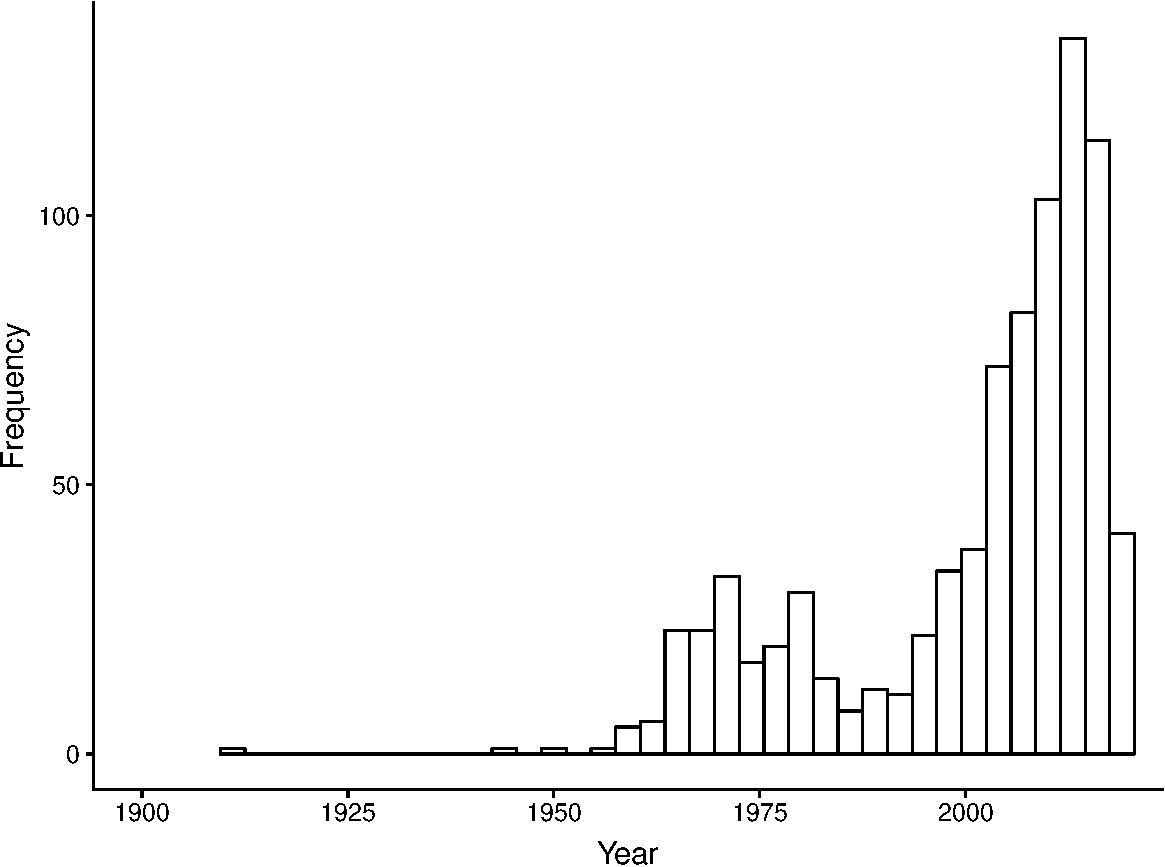
\includegraphics{LAB_files/figure-latex/pub-fig-1.pdf}
\caption{\label{fig:pub-fig}Overall publication frequency across years.}
\end{figure}

\hypertarget{stimuli}{%
\subsubsection{Stimuli}\label{stimuli}}

Stimuli are presented in Table \ref{tab:stim-table}, and a review of
this table indicated that the publication of word stimuli was the
largest category (38.2\%), followed by corpora (11.9\%). Other types of
word stimuli also appear commonly in the LAB data such as categories,
letters, and word pairs. Because linguistic data was of particular
interest, we selected publications based on words and word pairs, and
plotted the number of stimuli presented in the paper to examine big data
trends. These data were broken down by set size in Figure
\ref{fig:word-fig}. The upper left hand quadrant shows all stimuli
across years, and the big data publications stand out in the last
fifteen years of publications. We excluded two data points that included
over one million words to show the increase in publication of larger
datasets across years. This data was then further broken down into
smaller datasets (\textless{}10,000 stimuli; upper right quadrant), and
larger datasets (10,000+ stimuli; bottom left quadrant). The smaller
dataset graph shows that these publications are common across time,
while the bottom quadrant was more telling for the megastudies trend
investigation. As with languages and tags (below), we see an increase in
the number of larger datasets across the years.

\begin{figure}
\centering
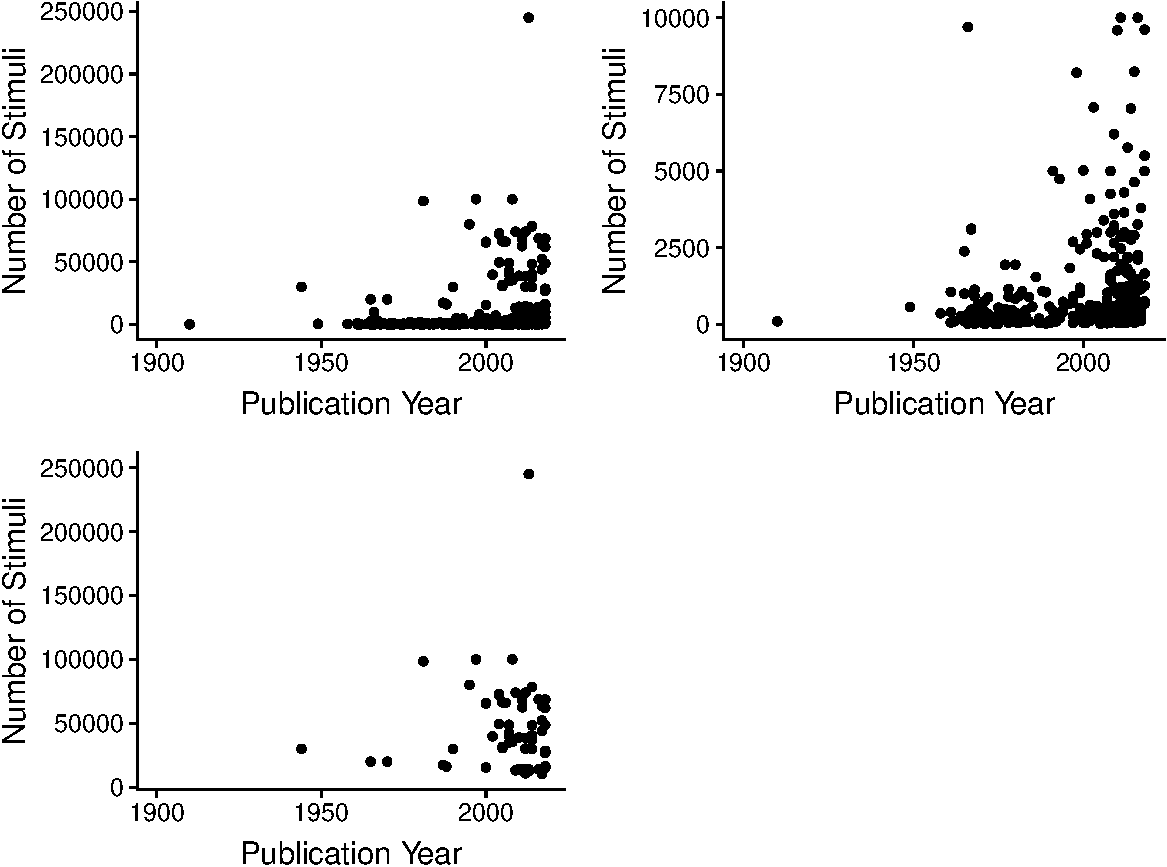
\includegraphics{LAB_files/figure-latex/word-fig-1.pdf}
\caption{\label{fig:word-fig}Number of word stimuli plotted across years.
Top left quandrant includes all word stimuli, minus two outliers. Top
right quadrant includes word stimuli ranging up to 10000 words, bottom
left quadrant portrays stimuli counts exceeding 10000. The x-axis is
consistent across graphs, however, the y-axis is scaled for the range of
stimuli targeted in that graph.}
\end{figure}

\hypertarget{languages}{%
\subsubsection{Languages}\label{languages}}

The variety and number of languages for stimuli provided a picture of
the growth and diversity of psycholinguistic stimuli, as seen in Table
\ref{tab:lang-table}. A growing number of articles include non-English
languages including Spanish ( 6.9\%), French ( 5.2\%), German ( 4.2\%),
and even include multiple languages ( 9.7\%). To examine trends, the
English only articles were filtered out of the dataset since they were
the majority of publications (53.2\%) and were published across all
years present in this data. Of the 389 non-English publications, 86
included multiple languages, and 45 of these were published after 2010.
Additionally, the last ten years (2008 and later) have seen an explosion
of publications in non-English languages: 256, with 32 in 2017 alone.
The publication of varied languages is still largely from WEIRD cultures
(Western Educated Industrialized Rich Democratic; Henrich, Heine, \&
Norenzayan, 2010) and Indo-European languages, thus, indicating room for
cross linguistic improvement.

\hypertarget{tags}{%
\subsubsection{Tags}\label{tags}}

\begin{figure}
\centering
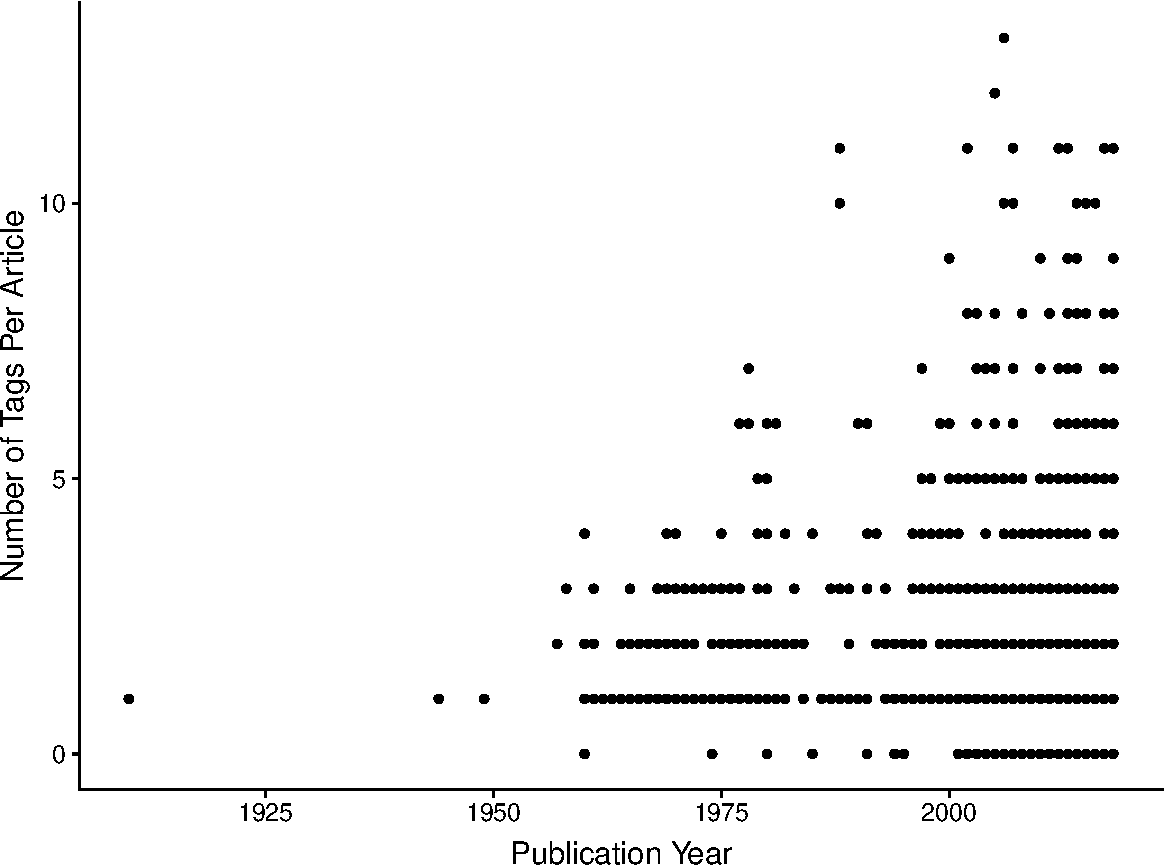
\includegraphics{LAB_files/figure-latex/tag-fig-1.pdf}
\caption{\label{fig:tag-fig}Number of tags included in each publication
across years.}
\end{figure}

Tables \ref{tab:tag-table} and \ref{tab:tag-table2} display the number,
percentages, correlations of tags across year for tags with sample sizes
greater than 10. Undoubtedly, these tags represent changes in
terminology over time, and some could be combined or recoined. However,
even if low frequency (\emph{N} \textless{}= 10; 11 tags in our dataset)
tags were excluded, 38 different tags were used to describe the types of
psycholinguistic data. Many of these tags can be considered individual
research areas, and the sizeable number of different options indicates
how complex and diverse the field has become since the publication of
free association norms in 1910 (Kent \& Rosanoff, 1910).

The total number of tags for each publication was then tallied, and this
data was plotted in Figure \ref{fig:tag-fig} to visualize if the number
of variables included in a study has grown over time (\emph{M} = 2.45,
\emph{SD} = 2.30). The correlation between total tags and year was
\(r = .17\), 95\% CI \([.10\), \(.23]\), \(t(843) = 4.90\),
\(p < .001\), indicating a small increase in total tags used over time.
Even considering the larger number of publications in the 2000s versus
1950s to 1970s, it appeared that the number of keywords for articles was
also slowly growing over time. This trend may indicate the evolution in
computing possibilities to be able to publish large amounts of data, but
also may indicate a desire to combine datasets so that even more stimuli
may be considered at once for modeling or experiment creation.

Next, tags with at least thirty publications were investigated
individually for trends across time (correlations presented in Tables
\ref{tab:tag-table} and \ref{tab:tag-table2}). Individual histograms can
be created by using the Tags Per Year area online, which show the total
frequency of the selected tag by year. Some small positive trends were
found, such as the increase in arousal, age of acquisition, syllables,
familiarity, and valence norms. Intriguingly, meaningfulness and
association both showed negative correlations, but these correlations
can be understood as an artifact of the publication of a book on
association norms in the 1970s (Postman \& Keppel, 1970), as well as a
recent drop off of in the small but steady use of meaningfulness. These
small correlations may partially be explained by the sheer number and
variation of data available in the LAB portal, as one would expect the
number of frequency tags to increase with the recent SUBTLEX
publications. Indeed, if the frequency tags were plotted by year an
increase across the last decade (18 in 2010, 15 in 2013, and 22 in 2014)
can be found. Readers are encouraged to view the individual graphs for
tags to investigate the change of keyword publication over time,
including the rise and demise of several research areas. For example,
confusion matrices heyday appeared to range from the early 70s to the
mid 80s, while arousal norms do not make a consistent appearance until
the late 90s.

\hypertarget{conclusion}{%
\section{Conclusion}\label{conclusion}}

This article had two main purposes: 1) to present the LAB dataset and
portal as an annotated bibliography and searchable tool for researchers,
and 2) to view trends in psycholinguistic research with an eye toward
big data. We believe the LAB website will be a useful channel for all
levels of researchers, from graduate students looking for experimental
stimuli to design their experiments, to the familiar investigator who
wishes to dig deeper into the diverse choices offered. The Language
Goldmine presents a similar resource, but the advantage to the LAB is
the breadth of publications coded, as well as the coding schema that
allowed for investigation of individual trends in publication. While the
majority of publications occur in one particular journal, the LAB allows
someone to find articles they may have missed in other areas with the
advantage of being collected into one location. User-friendly search
tools are provided to aide in searching for specific languages, stimuli,
or keywords, as well as multiple outputs for easy copying into Excel or
SPSS. While this article's statistics will become dated with the updates
to the LAB, dynamic tables and graphs are provided online to see the
current status of the field. Lastly, we encourage users to actively
report errors and suggest updates for the LAB dataset as a way to crowd
source information that is surely missing, especially in non-English
languages.

In the introduction, we provided two examples of current megastudies
(SUBTLEX and the Lexicon projects), in addition to how researchers might
collect big data through Mechanical Turk or Twitter. This article
focused on the breadth of the field to use the information provided by
publications as a window into the fluctuations of interest in areas.
Megastudies have become a prevalent topic, but data could have revealed
that this popularity was due to recent publication of a small subset of
articles. Instead, analyses showed that not only are the numbers of
publications accumulating, but the sizes of datasets are also growing in
tandem. Megastudies specifically focus on large datasets, but big data
can also be indicated here by the divergence in languages available,
number of places to publish such data, and the increasing number of
keywords for articles across years. Time will tell if these trends can
and will continue or if certain areas will see a confusion matrix type
decline after several large datasets are published. With the move of
traditional lab experiments to smartphone and tablet technology (Dufau
et al., 2011), it seems likely that researchers in psycholinguistics
will continue to find new and creative ways to modernize the field.

\newpage

\hypertarget{references}{%
\section{References}\label{references}}

\setlength{\parindent}{-0.5in}
\setlength{\leftskip}{0.5in}

\hypertarget{refs}{}
\leavevmode\hypertarget{ref-Adelman2006}{}%
Adelman, J. S., Brown, G. D., \& Quesada, J. F. (2006). Contextual
diversity, not word frequency, determines word-naming and lexical
decision times. \emph{Psychological Science}, \emph{17}(9), 814--823.
doi:\href{https://doi.org/10.1111/j.1467-9280.2006.01787.x}{10.1111/j.1467-9280.2006.01787.x}

\leavevmode\hypertarget{ref-R-papaja}{}%
Aust, F., \& Barth, M. (2017). \emph{papaja: Create APA manuscripts with
R Markdown}. Retrieved from \url{https://github.com/crsh/papaja}

\leavevmode\hypertarget{ref-Baayen1995}{}%
Baayen, R. H., Piepenbrock, R., Gulikers, L., \& Linguistic Data
Consortium. (1995). The CELEX lexical database (CD-ROM). Philidelphia.

\leavevmode\hypertarget{ref-Balota2004}{}%
Balota, D. A., Cortese, M. J., Sergent-Marshall, S. D., Spieler, D. H.,
\& Yap, M. J. (2004). Visual word recognition of single-syllable words.
\emph{Journal of Experimental Psychology: General}, \emph{133}(2),
283--316.
doi:\href{https://doi.org/10.1037/0096-3445.133.2.283}{10.1037/0096-3445.133.2.283}

\leavevmode\hypertarget{ref-Balota2007}{}%
Balota, D. A., Yap, M. J., Hutchison, K. A., Cortese, M. J., Kessler,
B., Loftis, B., \ldots{} Treiman, R. (2007). The English lexicon
project. \emph{Behavior Research Methods}, \emph{39}(3), 445--459.
doi:\href{https://doi.org/10.3758/BF03193014}{10.3758/BF03193014}

\leavevmode\hypertarget{ref-Barca2002}{}%
Barca, L., Burani, C., \& Arduino, L. S. (2002). Word naming times and
psycholinguistic norms for Italian nouns. \emph{Behavior Research
Methods, Instruments, \& Computers}, \emph{34}(3), 424--434.
doi:\href{https://doi.org/10.3758/BF03195471}{10.3758/BF03195471}

\leavevmode\hypertarget{ref-Boudelaa2010}{}%
Boudelaa, S., \& Marslen-Wilson, W. D. (2010). Aralex: A lexical
database for modern standard Arabic. \emph{Behavior Research Methods},
\emph{42}(2), 481--487.
doi:\href{https://doi.org/10.3758/BRM.42.2.481}{10.3758/BRM.42.2.481}

\leavevmode\hypertarget{ref-Bradshaw1984}{}%
Bradshaw, J. L. (1984). A guide to norms, ratings, and lists.
\emph{Memory \& Cognition}, \emph{12}(2), 202--206.
doi:\href{https://doi.org/10.3758/BF03198435}{10.3758/BF03198435}

\leavevmode\hypertarget{ref-Brodeur2010}{}%
Brodeur, M. B., Dionne-Dostie, E., Montreuil, T., \& Lepage, M. (2010).
The bank of standardized stimuli (BOSS), a new set of 480 normative
photos of objects to be used as visual stimuli in cognitive research.
\emph{PLoS ONE}, \emph{5}(5), e10773.
doi:\href{https://doi.org/10.1371/journal.pone.0010773}{10.1371/journal.pone.0010773}

\leavevmode\hypertarget{ref-Brysbaert2011}{}%
Brysbaert, M., Buchmeier, M., Conrad, M., Jacobs, A. M., Bölte, J., \&
Böhl, A. (2011). The word frequency effect: A review of recent
developments and implications for the choice of frequency estimates in
German. \emph{Experimental Psychology}, \emph{58}(5), 412--424.
doi:\href{https://doi.org/10.1027/1618-3169/a000123}{10.1027/1618-3169/a000123}

\leavevmode\hypertarget{ref-Brysbaert2009}{}%
Brysbaert, M., \& New, B. (2009). Moving beyond Kučera and Francis: A
critical evaluation of current word frequency norms and the introduction
of a new and improved word frequency measure for American English.
\emph{Behavior Research Methods}, \emph{41}(4), 977--990.
doi:\href{https://doi.org/10.3758/BRM.41.4.977}{10.3758/BRM.41.4.977}

\leavevmode\hypertarget{ref-Brysbaert2013}{}%
Brysbaert, M., Warriner, A. B., \& Kuperman, V. (2014). Concreteness
ratings for 40 thousand generally known English word lemmas.
\emph{Behavior Research Methods}, \emph{46}(3), 904--911.
doi:\href{https://doi.org/10.3758/s13428-013-0403-5}{10.3758/s13428-013-0403-5}

\leavevmode\hypertarget{ref-Buchanan2013}{}%
Buchanan, E. M., Holmes, J. L., Teasley, M. L., \& Hutchison, K. A.
(2013). English semantic word-pair norms and a searchable Web portal for
experimental stimulus creation. \emph{Behavior Research Methods},
\emph{45}(3), 746--757.
doi:\href{https://doi.org/10.3758/s13428-012-0284-z}{10.3758/s13428-012-0284-z}

\leavevmode\hypertarget{ref-Buchanan2018}{}%
Buchanan, E. M., \& Scofield, J. E. (2018). Methods to detect low
quality data and its implication for psychological research.
\emph{Behavior Research Methods}.
doi:\href{https://doi.org/10.3758/s13428-018-1035-6}{10.3758/s13428-018-1035-6}

\leavevmode\hypertarget{ref-Buhrmester2011}{}%
Buhrmester, M., Kwang, T., \& Gosling, S. D. (2011). Amazon's Mechanical
Turk: A new source of inexpensive, yet high-quality, data?
\emph{Perspectives on Psychological Science}, \emph{6}(1), 3--5.
doi:\href{https://doi.org/10.1177/1745691610393980}{10.1177/1745691610393980}

\leavevmode\hypertarget{ref-Burgess1998}{}%
Burgess, C., \& Livesay, K. (1998). The effect of corpus size in
predicting reaction time in a basic word recognition task: Moving on
from Kučera and Francis. \emph{Behavior Research Methods, Instruments,
and Computers}, \emph{30}(2), 272--277.
doi:\href{https://doi.org/10.3758/BF03200655}{10.3758/BF03200655}

\leavevmode\hypertarget{ref-Cai2010}{}%
Cai, Q., \& Brysbaert, M. (2010). SUBTLEX-CH: Chinese word and character
frequencies based on film subtitles. \emph{PLoS ONE}, \emph{5}(6),
e10729.
doi:\href{https://doi.org/10.1371/journal.pone.0010729}{10.1371/journal.pone.0010729}

\leavevmode\hypertarget{ref-R-shiny}{}%
Chang, W., Cheng, J., Allaire, J., Xie, Y., \& McPherson, J. (2017).
\emph{Shiny: Web application framework for r}. Retrieved from
\url{https://CRAN.R-project.org/package=shiny}

\leavevmode\hypertarget{ref-Cohen-Shikora2013}{}%
Cohen-Shikora, E. R., Balota, D. A., Kapuria, A., \& Yap, M. J. (2013).
The past tense inflection project (PTIP): Speeded past tense
inflections, imageability ratings, and past tense consistency measures
for 2,200 verbs. \emph{Behavior Research Methods}, \emph{45}(1),
151--159.
doi:\href{https://doi.org/10.3758/s13428-012-0240-y}{10.3758/s13428-012-0240-y}

\leavevmode\hypertarget{ref-Cree2003}{}%
Cree, G. S., \& McRae, K. (2003). Analyzing the factors underlying the
structure and computation of the meaning of chipmunk, cherry, chisel,
cheese, and cello (and many other such concrete nouns). \emph{Journal of
Experimental Psychology: General}, \emph{132}(2), 163--201.
doi:\href{https://doi.org/10.1037/0096-3445.132.2.163}{10.1037/0096-3445.132.2.163}

\leavevmode\hypertarget{ref-Cree1999}{}%
Cree, G. S., McRae, K., \& McNorgan, C. (1999). An attractor model of
lexical conceptual processing: Simulating semantic priming.
\emph{Cognitive Science}, \emph{23}, 371--414.
doi:\href{https://doi.org/10.1016/S0364-0213(99)00005-1}{10.1016/S0364-0213(99)00005-1}

\leavevmode\hypertarget{ref-Cuetos2011}{}%
Cuetos, F., Glez-Nosti, M., Barbon, A., \& Brysbaert, M. (2011).
SUBTLEX-ESP: Spanish word frequencies based on film subtitles.
\emph{Psicologica}, \emph{32}, 133--143.

\leavevmode\hypertarget{ref-DeDeyne2013}{}%
De Deyne, S., Navarro, D. J., \& Storms, G. (2013). Better explanations
of lexical and semantic cognition using networks derived from continued
rather than single-word associations. \emph{Behavior Research Methods},
\emph{45}(2), 480--498.
doi:\href{https://doi.org/10.3758/s13428-012-0260-7}{10.3758/s13428-012-0260-7}

\leavevmode\hypertarget{ref-Dimitropoulou2010}{}%
Dimitropoulou, M., Duñabeitia, J. A., Avilés, A., Corral, J., \&
Carreiras, M. (2010). Subtitle-based word frequencies as the best
estimate of reading behavior: The case of Greek. \emph{Frontiers in
Psychology}, \emph{1}(DEC), 1--12.
doi:\href{https://doi.org/10.3389/fpsyg.2010.00218}{10.3389/fpsyg.2010.00218}

\leavevmode\hypertarget{ref-Dodds2011}{}%
Dodds, P. S., Harris, K. D., Kloumann, I. M., Bliss, C. A., \& Danforth,
C. M. (2011). Temporal patterns of happiness and information in a global
social network: Hedonometrics and Twitter. \emph{PLoS ONE},
\emph{6}(12), e26752.
doi:\href{https://doi.org/10.1371/journal.pone.0026752}{10.1371/journal.pone.0026752}

\leavevmode\hypertarget{ref-Dufau2011}{}%
Dufau, S., Duñabeitia, J. A., Moret-Tatay, C., McGonigal, A., Peeters,
D., Alario, F. X., \ldots{} Grainger, J. (2011). Smart phone, smart
science: How the use of smartphones can revolutionize research in
cognitive science. \emph{PLoS ONE}, \emph{6}(9), e24974.
doi:\href{https://doi.org/10.1371/journal.pone.0024974}{10.1371/journal.pone.0024974}

\leavevmode\hypertarget{ref-Guasch2013}{}%
Guasch, M., Boada, R., Ferré, P., \& Sánchez-Casas, R. (2013). NIM: A
Web-based Swiss army knife to select stimuli for psycholinguistic
studies. \emph{Behavior Research Methods}, \emph{45}(3), 765--771.
doi:\href{https://doi.org/10.3758/s13428-012-0296-8}{10.3758/s13428-012-0296-8}

\leavevmode\hypertarget{ref-Glottolog}{}%
Hammarstrom, Forkel, \& Haspelmath. (n.d.). Glottolog 3.3. Retrieved
from \url{https://glottolog.org/}

\leavevmode\hypertarget{ref-Henrich2010}{}%
Henrich, J., Heine, S. J., \& Norenzayan, A. (2010). The weirdest people
in the world? \emph{Behavioral and Brain Sciences}, \emph{33}(2-3),
61--83.
doi:\href{https://doi.org/10.1017/S0140525X0999152X}{10.1017/S0140525X0999152X}

\leavevmode\hypertarget{ref-VanHeuven2014}{}%
Heuven, W. J. B. van, Mandera, P., Keuleers, E., \& Brysbaert, M.
(2014). Subtlex-UK: A New and Improved Word Frequency Database for
British English. \emph{Quarterly Journal of Experimental Psychology},
\emph{67}(6), 1176--1190.
doi:\href{https://doi.org/10.1080/17470218.2013.850521}{10.1080/17470218.2013.850521}

\leavevmode\hypertarget{ref-Hutchison2013}{}%
Hutchison, K. A., Balota, D. A., Neely, J. H., Cortese, M. J.,
Cohen-Shikora, E. R., Tse, C.-S., \ldots{} Buchanan, E. M. (2013). The
semantic priming project. \emph{Behavior Research Methods},
\emph{45}(4), 1099--1114.
doi:\href{https://doi.org/10.3758/s13428-012-0304-z}{10.3758/s13428-012-0304-z}

\leavevmode\hypertarget{ref-Kent1910a}{}%
Kent, G. H., \& Rosanoff, A. J. (1910). \emph{A study of association in
insanity} (Vol. 67, pp. 37--96). American Journal of Insanity.
doi:\href{https://doi.org/10.1037/13767-000}{10.1037/13767-000}

\leavevmode\hypertarget{ref-Keuleers2010}{}%
Keuleers, E., Brysbaert, M., \& New, B. (2010). SUBTLEX-NL: A new
measure for Dutch word frequency based on film subtitles. \emph{Behavior
Research Methods}, \emph{42}(3), 643--650.
doi:\href{https://doi.org/10.3758/BRM.42.3.643}{10.3758/BRM.42.3.643}

\leavevmode\hypertarget{ref-Keuleers2012}{}%
Keuleers, E., Lacey, P., Rastle, K., \& Brysbaert, M. (2012). The
British Lexicon Project: Lexical decision data for 28,730 monosyllabic
and disyllabic English words. \emph{Behavior Research Methods},
\emph{44}(1), 287--304.
doi:\href{https://doi.org/10.3758/s13428-011-0118-4}{10.3758/s13428-011-0118-4}

\leavevmode\hypertarget{ref-Kloumann2012}{}%
Kloumann, I. M., Danforth, C. M., Harris, K. D., Bliss, C. A., \& Dodds,
P. S. (2012). Positivity of the English language. \emph{PLoS ONE},
\emph{7}(1), e29484.
doi:\href{https://doi.org/10.1371/journal.pone.0029484}{10.1371/journal.pone.0029484}

\leavevmode\hypertarget{ref-Kucera1967}{}%
Kučera, H., \& Francis, W. N. (1967). \emph{Computational analysis of
present-day American English.} Providence, RI: Brown University Press.

\leavevmode\hypertarget{ref-Kuperman2012}{}%
Kuperman, V., Stadthagen-Gonzalez, H., \& Brysbaert, M. (2012).
Age-of-acquisition ratings for 30,000 English words. \emph{Behavior
Research Methods}, \emph{44}(4), 978--990.
doi:\href{https://doi.org/10.3758/s13428-012-0210-4}{10.3758/s13428-012-0210-4}

\leavevmode\hypertarget{ref-Landauer1997}{}%
Landauer, T. K., \& Dumais, S. T. (1997). A solution to Plato's problem:
The latent semantic analysis theory of acquisition, induction, and
representation of knowledge. \emph{Psychological Review}, \emph{104}(2),
211--240.
doi:\href{https://doi.org/10.1037//0033-295X.104.2.211}{10.1037//0033-295X.104.2.211}

\leavevmode\hypertarget{ref-Lete2004}{}%
Lété, B., Sprenger-Charolles, L., \& Colé, P. (2004). MANULEX: A
grade-level lexical database from French elementary school readers.
\emph{Behavior Research Methods, Instruments, \& Computers},
\emph{36}(1), 156--166.
doi:\href{https://doi.org/10.3758/BF03195560}{10.3758/BF03195560}

\leavevmode\hypertarget{ref-List}{}%
List, J.-M., Winter, B., \& Wedel, A. (n.d.). The Language Goldmine.
Retrieved from \url{http://languagegoldmine.com/}

\leavevmode\hypertarget{ref-Maki2004}{}%
Maki, W. S., McKinley, L. N., \& Thompson, A. G. (2004). Semantic
distance norms computed from an electronic dictionary (WordNet).
\emph{Behavior Research Methods, Instruments, \& Computers},
\emph{36}(3), 421--431.
doi:\href{https://doi.org/10.3758/BF03195590}{10.3758/BF03195590}

\leavevmode\hypertarget{ref-Mandera2015}{}%
Mandera, P., Keuleers, E., Wodniecka, Z., \& Brysbaert, M. (2015).
Subtlex-pl: subtitle-based word frequency estimates for Polish.
\emph{Behavior Research Methods}, \emph{47}(2), 471--483.
doi:\href{https://doi.org/10.3758/s13428-014-0489-4}{10.3758/s13428-014-0489-4}

\leavevmode\hypertarget{ref-Mason2012}{}%
Mason, W., \& Suri, S. (2012). Conducting behavioral research on
Amazon's Mechanical Turk. \emph{Behavior Research Methods},
\emph{44}(1), 1--23.
doi:\href{https://doi.org/10.3758/s13428-011-0124-6}{10.3758/s13428-011-0124-6}

\leavevmode\hypertarget{ref-McRae1997}{}%
McRae, K., Sa, V. R. de, \& Seidenberg, M. S. (1997). On the nature and
scope of featural representations of word meaning. \emph{Journal of
Experimental Psychology: General}, \emph{126}(2), 99--130.
doi:\href{https://doi.org/10.1037/0096-3445.126.2.99}{10.1037/0096-3445.126.2.99}

\leavevmode\hypertarget{ref-Miller2003}{}%
Miller, G. A. (2003). The cognitive revolution: A historical
perspective. \emph{Trends in Cognitive Sciences}, \emph{7}, 141--144.
doi:\href{https://doi.org/10.1016/S1364-6613(03)00029-9}{10.1016/S1364-6613(03)00029-9}

\leavevmode\hypertarget{ref-Moss2002}{}%
Moss, H. E., Tyler, L. K., \& Devlin, J. T. (2002). The emergence of
category-specific deficits in a distribuited semantic system. In E.
Forde \& G. Humphreys (Eds.), \emph{Category-specificity in mind and
brain} (pp. 115--145). CRC Press.

\leavevmode\hypertarget{ref-Nelson2004}{}%
Nelson, D. L., McEvoy, C. L., \& Schreiber, T. A. (2004). The University
of South Florida free association, rhyme, and word fragment norms.
\emph{Behavior Research Methods, Instruments, \& Computers},
\emph{36}(3), 402--407.
doi:\href{https://doi.org/10.3758/BF03195588}{10.3758/BF03195588}

\leavevmode\hypertarget{ref-New2007}{}%
New, B., Brysbaert, M., Veronis, J., \& Pallier, C. (2007). The use of
film subtitles to estimate word frequencies. \emph{Applied
Psycholinguistics}, \emph{28}(4), 661--677.
doi:\href{https://doi.org/10.1017/S014271640707035X}{10.1017/S014271640707035X}

\leavevmode\hypertarget{ref-Pexman2003}{}%
Pexman, P. M., Holyk, G. G., \& Monfils, M.-H. (2003).
Number-of-features effects and semantic processing. \emph{Memory \&
Cognition}, \emph{31}(6), 842--855.
doi:\href{https://doi.org/10.3758/BF03196439}{10.3758/BF03196439}

\leavevmode\hypertarget{ref-Postman1970}{}%
Postman, L., \& Keppel, G. (1970). \emph{Norms of word association.} New
York: Academic Press.

\leavevmode\hypertarget{ref-Proctor1999}{}%
Proctor, R. W., \& Vu, K.-P. L. (1999). Index of norms and ratings
published in the Psychonomic Society journals. \emph{Behavior Research
Methods, Instruments, \& Computers}, \emph{31}(4), 659--667.
doi:\href{https://doi.org/10.3758/BF03200742}{10.3758/BF03200742}

\leavevmode\hypertarget{ref-Rayner1986}{}%
Rayner, K., \& Duffy, S. A. (1986). Lexical complexity and fixation
times in reading: Effects of word frequency, verb complexity, and
lexical ambiguity. \emph{Memory \& Cognition}, \emph{14}(3), 191--201.
doi:\href{https://doi.org/10.3758/BF03197692}{10.3758/BF03197692}

\leavevmode\hypertarget{ref-Rogers2004}{}%
Rogers, T. T., \& McClelland, J. L. (2004). \emph{Semantic cognition: A
parallel distributed processing approach}. MIT Press.

\leavevmode\hypertarget{ref-Snodgrass1980}{}%
Snodgrass, J. G., \& Vanderwart, M. (1980). A standardized set of 260
pictures: Norms for name agreement, image agreement, familiarity, and
visual complexity. \emph{Journal of Experimental Psychology: Human
Learning and Memory}, \emph{6}(2), 174--215.
doi:\href{https://doi.org/10.1037/0278-7393.6.2.174}{10.1037/0278-7393.6.2.174}

\leavevmode\hypertarget{ref-Soares2014}{}%
Soares, A. P., Medeiros, J. C., Simões, A., Machado, J., Costa, A.,
Iriarte, Á., \ldots{} Comesaña, M. (2014). ESCOLEX: A grade-level
lexical database from European Portuguese elementary to middle school
textbooks. \emph{Behavior Research Methods}, \emph{46}(1), 240--253.
doi:\href{https://doi.org/10.3758/s13428-013-0350-1}{10.3758/s13428-013-0350-1}

\leavevmode\hypertarget{ref-Sze2014}{}%
Sze, W. P., Rickard Liow, S. J., \& Yap, M. J. (2014). The Chinese
Lexicon Project: A repository of lexical decision behavioral responses
for 2,500 Chinese characters. \emph{Behavior Research Methods},
\emph{46}(1), 263--273.
doi:\href{https://doi.org/10.3758/s13428-013-0355-9}{10.3758/s13428-013-0355-9}

\leavevmode\hypertarget{ref-Tse2017}{}%
Tse, C.-S., Yap, M. J., Chan, Y.-L., Sze, W. P., Shaoul, C., \& Lin, D.
(2017). The Chinese Lexicon Project: A megastudy of lexical decision
performance for 25,000+ traditional Chinese two-character compound
words. \emph{Behavior Research Methods}, \emph{49}(4), 1503--1519.
doi:\href{https://doi.org/10.3758/s13428-016-0810-5}{10.3758/s13428-016-0810-5}

\leavevmode\hypertarget{ref-Vaughan2004}{}%
Vaughan, J. (2004). A web-based archive of norms, stimuli, and data.
\emph{Behavior Research Methods, Instruments, \& Computers},
\emph{36}(3), 363--370.
doi:\href{https://doi.org/10.3758/BF03195583}{10.3758/BF03195583}

\leavevmode\hypertarget{ref-Vigliocco2004}{}%
Vigliocco, G., Vinson, D. P., Lewis, W., \& Garrett, M. F. (2004).
Representing the meanings of object and action words: The featural and
unitary semantic space hypothesis. \emph{Cognitive Psychology},
\emph{48}(4), 422--488.
doi:\href{https://doi.org/10.1016/j.cogpsych.2003.09.001}{10.1016/j.cogpsych.2003.09.001}

\leavevmode\hypertarget{ref-Vinson2003}{}%
Vinson, D. P., Vigliocco, G., Cappa, S., \& Siri, S. (2003). The
breakdown of semantic knowledge: Insights from a statistical model of
meaning representation. \emph{Brain and Language}, \emph{86}(3),
347--365.
doi:\href{https://doi.org/10.1016/S0093-934X(03)00144-5}{10.1016/S0093-934X(03)00144-5}

\leavevmode\hypertarget{ref-Vo2009}{}%
Vo, M. L. H., Conrad, M., Kuchinke, L., Urton, K., Hofmann, M. J., \&
Jacobs, A. M. (2009). The Berlin Affective Word List Reloaded (BAWL-R).
\emph{Behavior Research Methods}, \emph{41}(2), 534--538.
doi:\href{https://doi.org/10.3758/BRM.41.2.534}{10.3758/BRM.41.2.534}

\leavevmode\hypertarget{ref-Warriner2013}{}%
Warriner, A. B., Kuperman, V., \& Brysbaert, M. (2013). Norms of
valence, arousal, and dominance for 13,915 English lemmas.
\emph{Behavior Research Methods}, \emph{45}(4), 1191--1207.
doi:\href{https://doi.org/10.3758/s13428-012-0314-x}{10.3758/s13428-012-0314-x}

\leavevmode\hypertarget{ref-Yap2010}{}%
Yap, M. J., Rickard Liow, S. J., Jalil, S. B., \& Faizal, S. S. B.
(2010). The Malay lexicon project: A database of lexical statistics for
9,592 words. \emph{Behavior Research Methods}, \emph{42}(4), 992--1003.
doi:\href{https://doi.org/10.3758/BRM.42.4.992}{10.3758/BRM.42.4.992}

\leavevmode\hypertarget{ref-Yap2011}{}%
Yap, M. J., Tan, S. E., Pexman, P. M., \& Hargreaves, I. S. (2011). Is
more always better? Effects of semantic richness on lexical decision,
speeded pronunciation, and semantic classification. \emph{Psychonomic
Bulletin and Review}, \emph{18}(4), 742--750.
doi:\href{https://doi.org/10.3758/s13423-011-0092-y}{10.3758/s13423-011-0092-y}

\leavevmode\hypertarget{ref-Zevin2002}{}%
Zevin, J., \& Seidenberg, M. (2002). Age of acquisition effects in word
reading and other tasks. \emph{Journal of Memory and Language},
\emph{47}(1), 1--29.
doi:\href{https://doi.org/10.1006/jmla.2001.2834}{10.1006/jmla.2001.2834}


\end{document}
